\chapter{Network configuration}

Hazelcast can run perfectly within a single JVM and this is excellent for development and to speed up testing. But Hazelcast true strength becomes apparent when a cluster of JVM's running on multiple machines is created. Having a cluster of machines makes Hazelcast resilient to failure; if one machine fails, the data will failover to another machine as if nothing happened. It also makes Hazelcast scalable; just add extra machines to the cluster, to gain additional capacity. Creating clusters can be done by configuring the network settings.

To test the networking settings, we are going to make use of the following minimalistic Hazelcast member unless specified otherwise:
\begin{lstlisting}[language=java]
public class Member {
   public static void main(String[] args) {
      Hazelcast.newHazelcastInstance();
   }
}
\end{lstlisting}
In this chapter we are going to rely on the hazelcast.xml config file to set the networking options:
\begin{lstlisting}[language=xml]
<hazelcast>
   ...
   <network>
      ...  
   </network>
   ...
</hazelcast>
\end{lstlisting}

\section{Port}
One of the most basic configuration settings is the port Hazelcast is going to use for communication between the members. This can be done by the 'port' property in the network configuration which defaults to 5701. If the port is already in use and if auto-increment property is true, which is the default, Hazelcast will automatically try to find next free port, example:
\begin{lstlisting}[language=xml]
<network>
    <port auto-increment="true">5701</port>
</network>
\end{lstlisting}
If you start the member, you will get output like:
\begin{lstlisting}
INFO: [192.168.1.101]:5701 [dev] Address[192.168.1.101]:5701 is STARTED
\end{lstlisting}
As you can see, the port 5701 is being used. If another member is started, you will see that port 5702 is assigned. If you look carefully at the end of the logging, you'll see a warning about cluster size is 1. The cause of this is that the created members don't form a cluster but are standalone. To create a cluster you need to configure a join mechanism.

\section{Join Mechanism }
Hazelcast supports 3 mechanisms for members to join the cluster: multicast, tcp/ip-cluster, Amazon EC2 and one of these mechanism needs to be enabled to form a cluster, else they will remain standalone. Make sure that only 1 join mechanism is enabled. After joining the cluster, Hazelcast relies on TCP for internal communication. Also make sure that only a single join mechanism is enabled.

\subsection{Multicast}
With multicast discovery a member will send a message to all members that listen on a specific multicast group. It is the easiest mechanism to use, but is not always available. Underneath you can see a very minimalistic multicast configuration:
\begin{lstlisting}[language=xml]
<network>
   <join><multicast enabled="true"/></join>
</network>
\end{lstlisting}
If you start one member, you will see output like this:
\begin{lstlisting}
Jan 22, 2013 2:06:30 PM com.hazelcast.impl.MulticastJoiner
INFO: [192.168.1.104]:5701 [dev] 

Members [1] {
   Member [192.168.1.104]:5701 this
}
\end{lstlisting}	
As you can see, the member is started and currently the cluster has a single member. If you start another member on the same machine, on the console of the first member the following will be added to the output:
\begin{lstlisting}
Members [2] {
   Member [192.168.1.104]:5701 this
   Member [192.168.1.104]:5702
}
\end{lstlisting}	
As you can see, the first member can see the second member. And if we look at the end of logging for the second member, we'll find something similar:
\begin{lstlisting}
Members [2] {
   Member [192.168.1.104]:5701
   Member [192.168.1.104]:5702 this
}
\end{lstlisting}		
We now have a 2 member Hazelcast cluster running on a single machine. It starts to become more interesting if you start multiple members on different machines.

The multicast configuration can be tuned using the following attributes:
\begin{enumerate}
\item multicast-group: With multicast a member is part of the multicast group and will not receive multicast messages from other group. So by setting the multicast-group or the multicast-port, you can have separate Hazelcast clusters within the same network and it is a best practice to use separate groups if the same network is used for different purposes. The multicast group ip address doesn't conflict with normal unicast ip addresses since they have a specific range that is excluded from normal unicast usage: 224.0.0.0 to 239.255.255.255 (inclusive) and defaults:224.2.2.3. The address 224.0.0.0 is reserved and should not be used.   
\item multicast-port: The port of the multicast socket where the Hazelcast member listens and sends discovery messages to. Unlike normal unicast sockets where only a single process can listen to a port, with multicast sockets multiple processes can listen to the same port. So you don't need to be worried about having multiple Hazelcast members that run on the same JVM are going to conflict. This property defaults to 54327
\item multicast-time-to-live-seconds: Set the default time-to-live for multicast packets sent out on this in order to control the scope of the multicasts. Defaults to 32 and a maximum of 255.
\item multicast-timeout-seconds:defaults:2: [todo: property of hazelcast, when to give up to find a master.]
\item trusted-interfaces:[todo]it defines who to trust; so you can list the interfaces that are good and responses from no good 'interfaces' will be prevented.
\end{enumerate}

\subsubsection{Debugging multicast}
If you don't see members joining, then it is likely because multicast is not available. A cause can be the firewall; you can test this by disabling the firewall or enable multicast in the firewall [see firewall section]. Another cause can be that it is disabled on the network or the network doesn't support it. On *NIX environments you can check if your network interface supports multicast by calling 'ifconfig | grep -i multicast', but it doesn't mean that it is available. To check if multicast is available, 'iperf' is a useful tool which is available for Windows/*NIX/OSX. To test multicast using multicast-group '224.2.2.3', open a terminal one 2 machines within the network and run the following in the first terminal 'iperf -s -u -B 224.2.2.3 -i 1' and 'iperf -c 224.2.2.3 -u -T 32 -t 3 -i 1' in the other terminal. If data is being transferred then multicast is working.

If you want to use multicast for local development and it isn't working, you can try the following unicast configuration:
\begin{lstlisting}[language=xml]
<network>
   <join>
      <multicast enabled="false"/>
      <tcp-ip enabled="true"/>
   </join>
</network>
\end{lstlisting}

\subsection{TCP/IP cluster}
In the previous section we made use of multicast, but this is not always an option because in production environments it often is prohibited and in cloud environments it often is not supported. That is why there is another discovery mechanism: the TCP/IP cluster. The idea is that there should be a one or more well known members to connect to. Once members have connected to these well known members and joined the cluster, they will keep each other up to date with all member addresses.

Underneath is an example of a TCP/IP cluster configuration where such a well known member with IP '192.168.1.104':
\begin{lstlisting}[language=xml]
<network>
   <join>
      <multicast enabled="false"/>
      <tcp-ip enabled="true">
         <member>192.168.1.104</member> 
      </tcp-ip>
   </join>
</network>
\end{lstlisting}
Multiple members can be configured using a comma or semicolon separated list, or multiple '<member>' entries. A range of IP's can be defined using syntax '192.168.1.100-200'. If no port is provided, Hazelcast will automatically try port 5701..5703 [todo: starts from the configured port]. If depending on IP addresses is not desirable, it also is possible to provide the hostname. Instead of using multiple '<member>' you can also use '<members>', but it doesn't change the meaning of the configuration. 

By default Hazelcast will 'bind' (so accept incoming traffic) to all local network interfaces. If this is unwanted behavior the 'hazelcast.socket.bind.any' [todo:hazelcast.server.socket.bind.any/hazelcast.client.socket.bind.any.] can be set to false. In that case Hazelcast will first use the interfaces configured in the 'interfaces/interfaces' to resolve one interface to bind to. If none is found, it will use the interfaces in the 'tcp-ip/members' to resolve one interface to bind to. If no interface is found, it will default to localhost.

When there is a large number of IP's listed [todo: especially in virtualized environments] and members can't build up a cluster, the 'conn-timeout-seconds' attribute, which defaults to 5, can be set to a higher value. The first scan and delay between scans can be configured using property 'hazelcast.merge.first.run.delay.seconds' and respectively 'hazelcast.merge.next.run.delay.seconds'. By default Hazelcast will scan every 5 seconds.

\subsection{EC2 Auto Discovery}
Apart from multicast and the tcp/ip-cluster join mechanisms, there a third mechanism: Amazon EC2. This mechanism, which makes use of tcp/ip discovery behind the scenes, sees all nodes within a particular region and have certain tag keys/values, as well known members. So a single region is used to lets new nodes discover the cluster, but the cluster can span multiple regions (it can even span multiple cloud providers).

So lets start with a very simple setup:
\begin{lstlisting}[language=xml]
<network>
   <join>
      <multicast enabled="false"/>
      <aws enabled="true">
         <access-key>my-access-key</access-key>
         <secret-key>my-secret-key</secret-key>
      </aws>
   </join>
</network>
\end{lstlisting}
And 'my-access-key' and 'my-secret-key' need to be replaced with your access key and secret key. Make sure that the started machines have a security group where the correct ports are opened (see firewall).

The AWS section also has a few configuration options:
\begin{enumerate}
\item region: the region where the machines are running. Defaults to 'us-east-1'.
\item tag-key,tag-value: allows you to limit the numbers of machines to look at by providing them with a unique tag-key/tag-value. This makes it possible to create multiple cluster in a single data center.
\item security-group-name: just like the tag-key,tag-value, it filters out machines. Doesn't need to be specified.
\end{enumerate}
And the aws tag accepts an attribute called "conn-timeout-seconds". The default value is 5 and can be increased  if you have many IP's listed and members can not properly build up the cluster.

In case you are using a different cloud provider than Amazon EC2, you can still make use of Hazelcast. What you can do it to use the programmatic api to configure a tcp-ip cluster and the well known members need to be retrieved from your cloud provider (e.g. using jclouds).

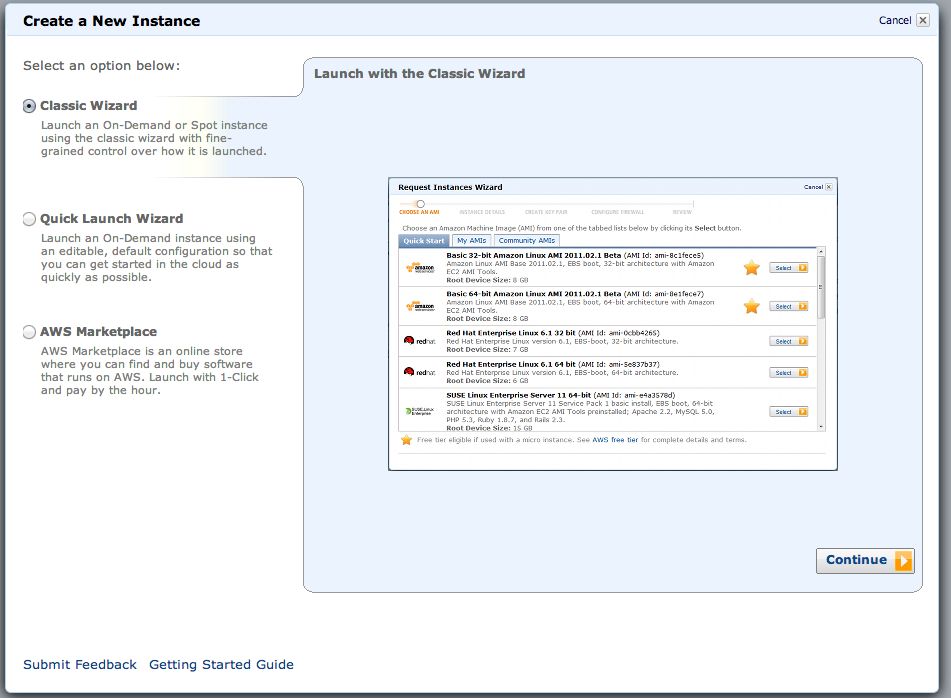
\includegraphics[scale=0.40]{ec2-1.png}

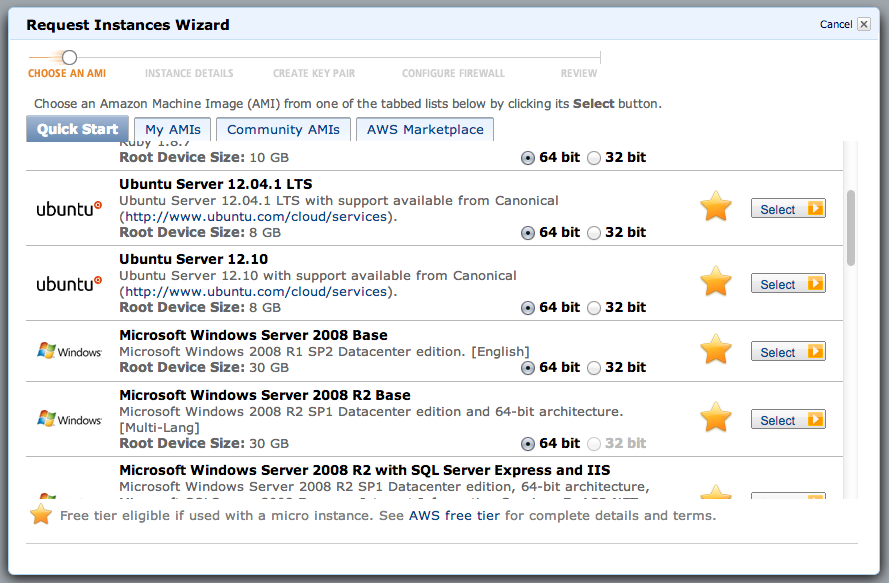
\includegraphics[scale=0.40]{ec2-2.png}

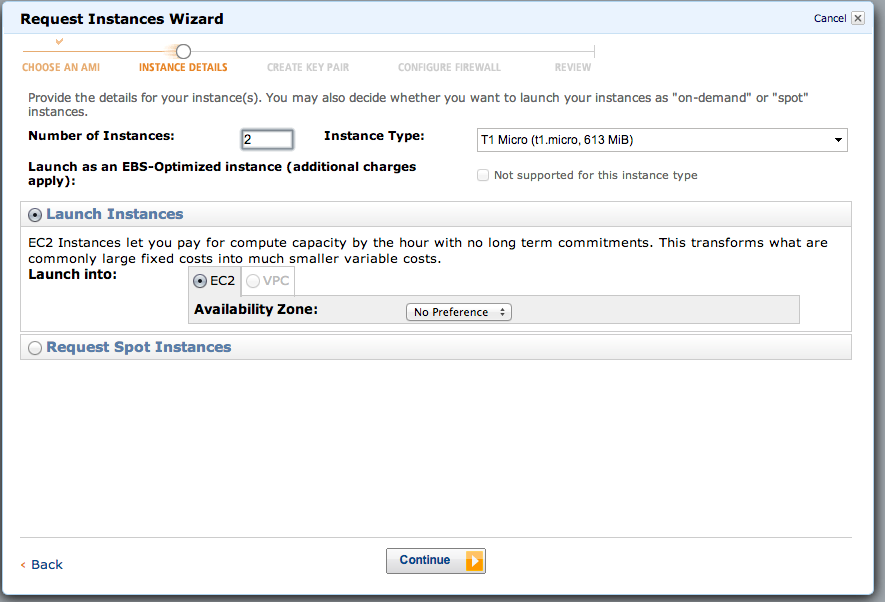
\includegraphics[scale=0.40]{ec2-3.png}

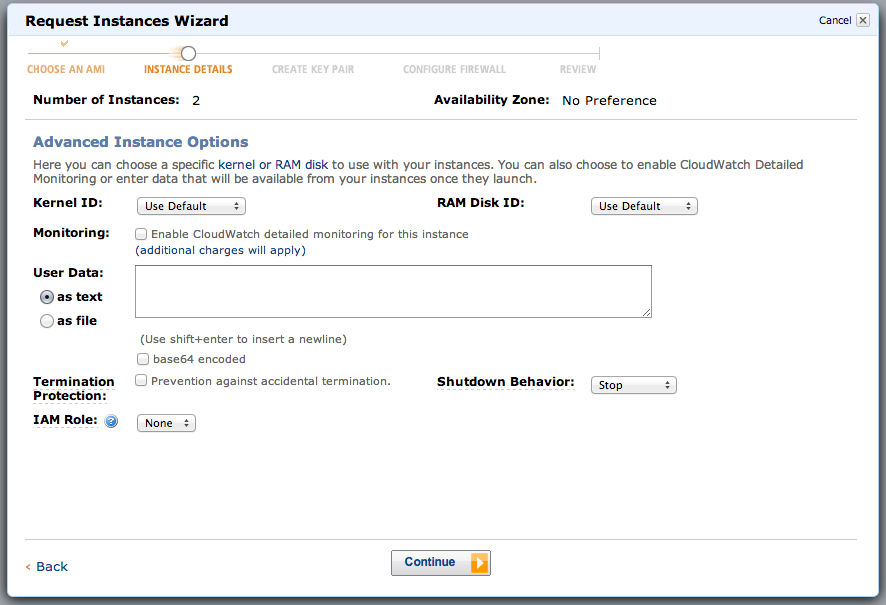
\includegraphics[scale=0.40]{ec2-4.png}

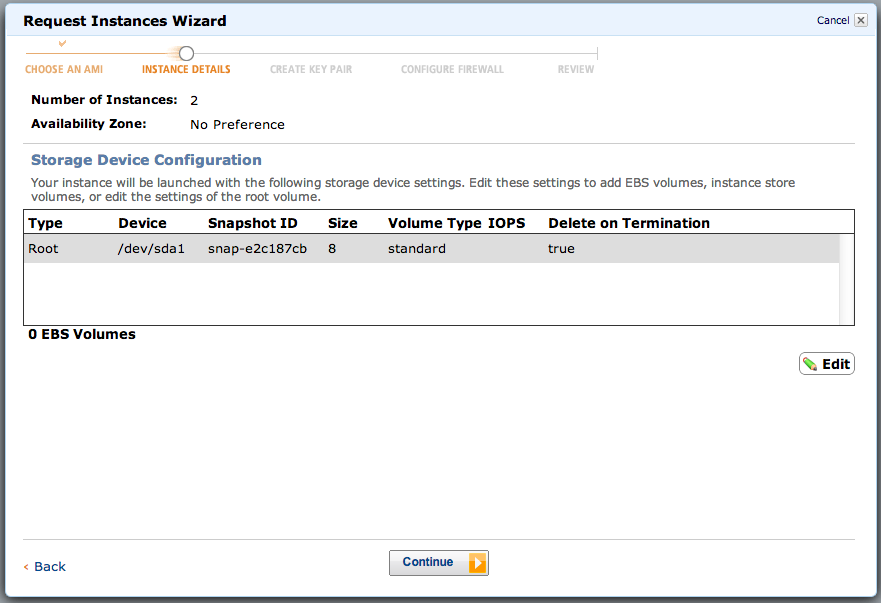
\includegraphics[scale=0.40]{ec2-5.png}

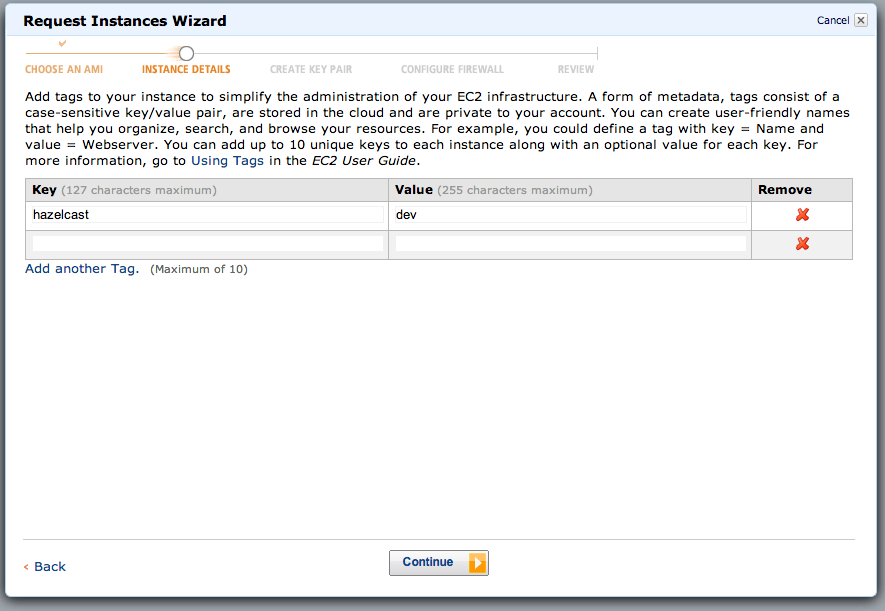
\includegraphics[scale=0.40]{ec2-6.png}

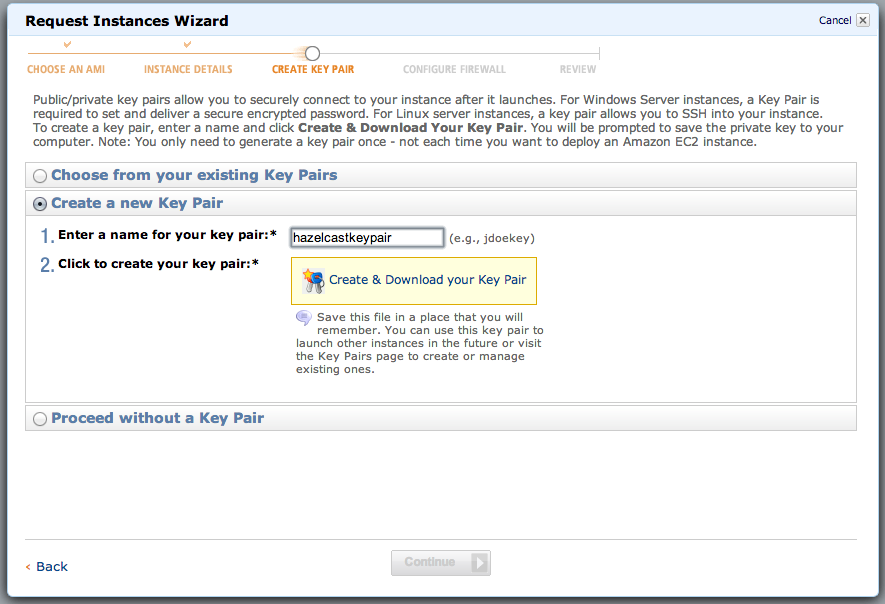
\includegraphics[scale=0.40]{ec2-7.png}

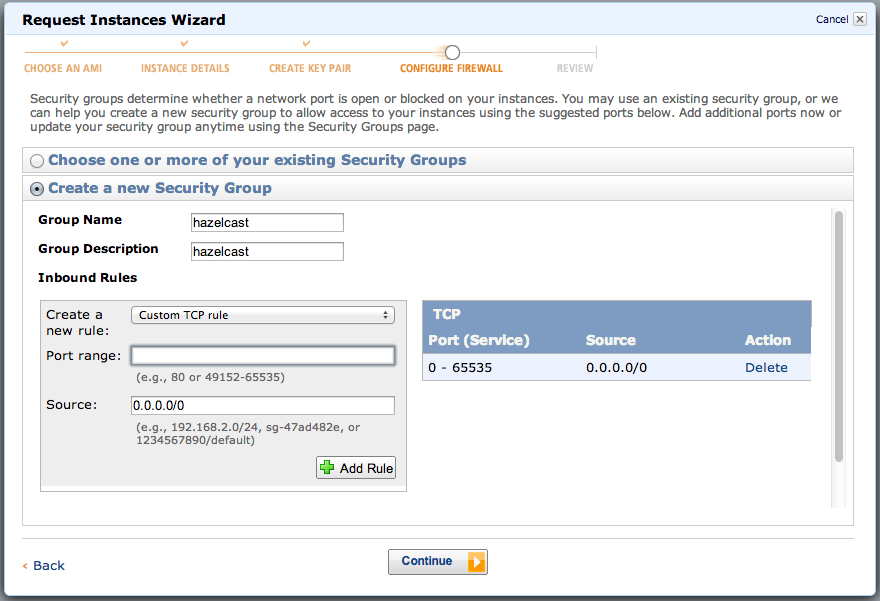
\includegraphics[scale=0.40]{ec2-8.png}

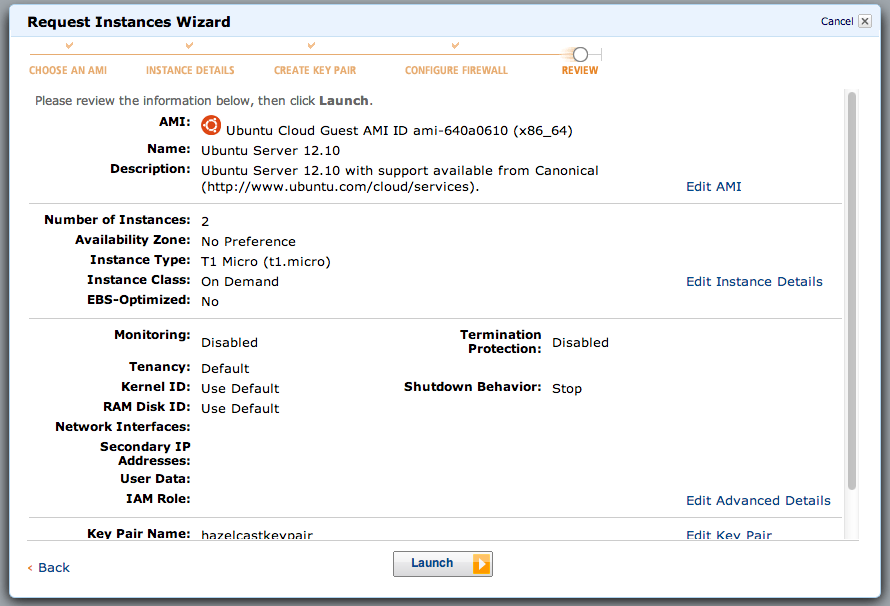
\includegraphics[scale=0.40]{ec2-9.png}

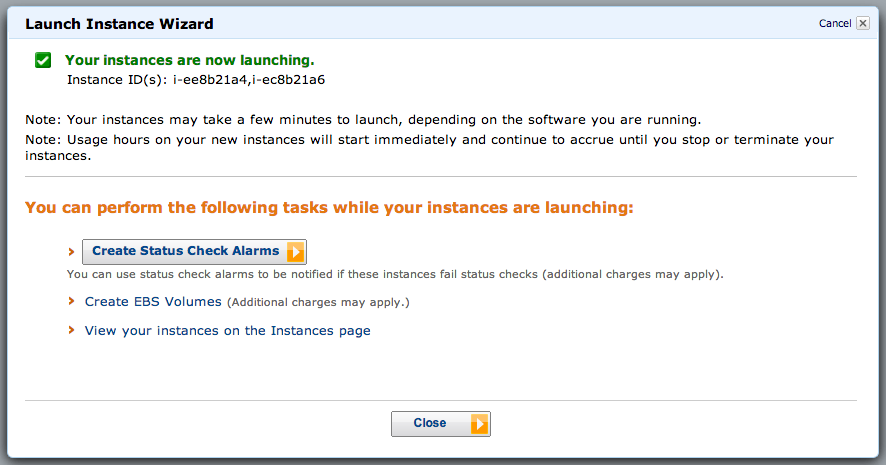
\includegraphics[scale=0.40]{ec2-10.png}

\section{Partition Group Configuration}
Normally Hazelcast prevents the master and the backup partitions to be stored on the same JVM to guarantee high availability. But it can be that multiple Hazelcast members of the same cluster are running on the same machine; so when the machine fails it can still happen that both master and backup fail. Luckily Hazelcast provides a solution for this problem in the form of partition groups:
\begin{lstlisting}[language=xml]
<hazelcast>
   <partition-group enabled="true" group-type="HOST_AWARE"/>
</hazelcast>
\end{lstlisting}
Using this configuration all members that share the same hostname/host-IP, will be part of the same group and therefor will not host both master and backup(s). [todo: what happens when there are no other members?] 

Another reason partition groups can be useful is that normally Hazelcast considers all machines to be equal and therefor will distribute the partitions evenly. But in some cases machines are not equal, e.g. different amount of memory available or slower cpu's, so could lead to a load imbalance. With a partition group you can make member-groups where each member-group is considered to have the same capacity and where each member is considered to have the same capacity as the other members in the same member-group. In the future perhaps a balance-factor will be added to relax these constraints. Underneath is an example where we define multiple member groups based on matching ip-addresses:
\begin{lstlisting}[language=xml]
<hazelcast>
   <partition-group enabled="true" group-type="CUSTOM">
      <member-group>
         <interface>10.10.1.*</interface>
      </member-group>
      <member-group>
         <interface>10.10.2.*</interface>
      </member-group
   </partition-group>
</hazelcast>
\end{lstlisting}
In this example there are 2 member groups, where the first member-group contains all member with an IP 10.10.1.0-255 and the second member-group contains all member with an IP of 10.10.2.0-255. You can also this approach to create different groups for each data-center so that when the primary datacenter goes offline, the backup datacenter can take over.

\section{Creating Separate Clusters}
Sometimes it desirable to have multiple isolated clusters on the same network instead of a single cluster. For example when a network is used for different environments or different applications. Luckily this can be done using groups:
\begin{lstlisting}[language=xml]
<hazelcast>
   <group>
      <name>application1</name>
      <password>somepassword</password>
   </group>
</hazelcast>
\end{lstlisting}
The password is optional and defaults to 'dev-pass'. A group is something else than a partition-group; with the former you create isolated clusters and with the latter you control how partitions are being mapped to members.

\section{SSL}
In a production environment often you want to prevent that the communication between Hazelcast members can be tampered or can be read, with ... because it could contains sensitive information. Luckily Hazelcast provides a solution for that: SSL encryption.

The basic functionality is provided by 'com.hazelcast.nio.ssl.SSLContextFactory' interface and configurable through the the SSL section in network configuration. Luckily Hazelcast provides a default implementation called the 'com.hazelcast.nio.ssl.BasicSSLContextFactory' which we are going to use for the example:
\begin{lstlisting}[language=xml]
<network>
   <join><multicast enabled="true"/></join>
   <ssl enabled="true">
      <factory-class-name>com.hazelcast.nio.ssl.BasicSSLContextFactory</factory-class-name>
      <properties>
         <property name="keyStore">keyStore.jks</property>
         <property name="keyStorePassword">password</property>
      </properties>
   </ssl>
</network>
\end{lstlisting}
The 'keyStore' is the path to the keyStore. [todo: is it possible to provide a classpath reference so it can be included in the jar, and is this a desirable practice?] and the 'keyStorePassword' is the password of the keystore. In the example code you can find an already created keystore and also the documentation to create one yourself.

When you start a member, you will see that SSL is enabled:
\begin{lstlisting}
INFO: [192.168.1.104]:5701 [dev] SSL is enabled
\end{lstlisting}

There are some additional properties that can be set on the BasicSSLContextFactory:
\begin{enumerate}
\item keyManagerAlgorithm: defaults to 'SunX509'.
\item trustManagerAlgorithm: defaults to 'SunX509'.
\item protocol: defaults to 'TLS'
\end{enumerate}
Another way to configure the keyStore/keyStorePassword is through the 'javax.net.ssl.keyStore' and 'javax.net.ssl.keyStorePassword' system properties. The recommended practice is to make a single keyStore file that is shared between all instances. It isn't possible to include the keystore within the jar.

\section{Encryption}
Apart from supporting SSL, Hazelcast also supports symmetric encryption based on the Java Cryptography Architecture (JCA). The main advantage of using the latter is that it is easier to set up because you don't need to deal with the keystore. The main disadvantage is that its less secure, because SSL relies on an on the fly created public/private key pair and the symmetric encryption relies on a constant password/salt.

SSL and symmetric encryption solutions will roughly have the same CPU and network bandwidth overhead since for the main data  they rely on symmetric encryption (only the public key is encrypted using asymmetric encryption). Compared to non encrypted data, the performance degradation will be roughly 50%. [todo: increased latency]

The demonstrate the encryption, lets have a look at the following configuration:
\begin{lstlisting}[language=xml]
<network>
   <join><multicast enabled="true"/></join>
   <symmetric-encryption enabled="true">
      <algorithm>PBEWithMD5AndDES</algorithm>
      <salt>somesalt</salt>
      <password>somepass</password>
      <iteration-count>19</iteration-count>
   </symmetric-encryption>
</network>
\end{lstlisting}
When we start 2 members using this configuration, we'll see that the symmetric encryption is activated:
\begin{lstlisting}
Jan 20, 2013 9:22:08 AM com.hazelcast.nio.SocketPacketWriter
INFO: [192.168.1.104]:5702 [dev] Writer started with SymmetricEncryption
Jan 20, 2013 9:22:08 AM com.hazelcast.nio.SocketPacketReader
INFO: [192.168.1.104]:5702 [dev] Reader started with SymmetricEncryption
\end{lstlisting}

Since encryption relies on the JCA, additional algorithms can be used by enabling the Bouncy Castle JCA provider through property 'hazelcast.security.bouncy.enabled'. Hazelcast used to have support for asymmetric encryption, but due its complex setup, this feature has been removed from Hazelcast 3.0. Currently there is no support for encryption between a native client and a cluster member.

\section{Firewall}
When a Hazelcast member connects to another Hazelcast member, it binds to server port 5701 (see the port configuration section) to receive the inbound traffic. On the client side also a port needs to be opened for the outbound traffic. By default this will be an 'ephemeral' port since we it doesn't matter which port is being used as long as it is free. The problem is that the lack of control on the outbound port, can be a security issues, because the firewall needs to expose all ports for outbound traffic. 

Luckily Hazelcast is able to control the outbound ports. For example if we want to allow the port range 30000-31000, it can be configured like this:
\begin{lstlisting}[language=xml]
<network>
   <join><multicast enabled="true"/></join>
   <outbound-ports>
      <ports>30000-31000</ports>
   </outbound-ports>
</network>
\end{lstlisting}
To demonstrate the outbound ports configuration, start 2 Hazelcast members with this configuration and when the members are fully started, execute 'sudo lsof -i | grep java'. Below you can see the cleaned output of the command:
\begin{lstlisting}
java 46117 IPv4 TCP *:5701 (LISTEN)
java 46117 IPv4 TCP 172.16.78.1:5701->172.16.78.1:30609 (ESTABLISHED)
java 46120 IPv4 TCP *:5702 (LISTEN)
java 46120 IPv4 TCP 172.16.78.1:30609->172.16.78.1:5701 (ESTABLISHED)
\end{lstlisting}
As you can see there are 2 java processes: 46117 and 46120 that listen on port 5701 and 5702 (inbound traffic). You can also see that java process 46120 is using port 30609 for outbound traffic.

Apart from specifying port ranges, you can also specify individual ports. Multiple port configurations can be combined either by separating them by comma or by providing multiple '<ports>' sections. So if you want to use port 30000,30005 and portrange 31000 till 32000, you could say the following '<ports>30000,30005,31000-32000</ports>'. 

\subsection{iptables}
If you are making use of iptables, the following rule can be added to allow for outbound traffic from ports 33000-31000:
\begin{lstlisting}
iptables -A OUTPUT -p TCP --dport 33000:31000 -m state --state NEW -j ACCEPT
\end{lstlisting}
and to control incoming traffic from any address to port 5701:
\begin{lstlisting}
iptables -A INPUT -p tcp -d 0/0 -s 0/0 --dport 5701 -j ACCEPT
\end{lstlisting}
and to allow incoming multicast traffic:
\begin{lstlisting}
iptables -A INPUT -m pkttype --pkt-type multicast -j ACCEPT
\end{lstlisting}

\section{Specifying network interfaces}
Most server machines can have multiple network interfaces. 

You can also specify which network interfaces that Hazelcast should use. Servers mostly have more than one network interface so you may want to list the valid IPs. Range characters ('*' and '-') can be used for simplicity. So 10.3.10.*, for instance, refers to IPs between 10.3.10.0 and 10.3.10.255. Interface 10.3.10.4-18 refers to IPs between 10.3.10.4 and 10.3.10.18 (4 and 18 included). If network interface configuration is enabled (disabled by default) and if Hazelcast cannot find an matching interface, then it will print a message on console and won't start on that member.

\begin{lstlisting}[language=xml]
<hazelcast>
    <network>
        <interfaces enabled="true">
            <interface>10.3.16.*</interface> 
            <interface>10.3.10.4-18</interface> 
            <interface>192.168.1.3</interface>         
        </interfaces>    
    </network>
</hazelcast>
\end{lstlisting}

[todo: when there are multiple interfaces, which is selected by default?]
[todo: does this work for multicast?]
[todo: every machine could have different interfaces. So should all the interfaces be listed of all machines? Or should an hazelcast config per machine be 'generated'?]

\section{What is next}
The network configuration for Hazelcast is very extensive. There are some features like IPv6,  network partitioning (split-brain syndrome), specifying network interfaces, socket interceptors, WAN replication, that have been left out, but can be found on the Hazelcast reference manual. Also the mailing-list is a very valuable source of information.

